\documentclass{subfiles}

\begin{document}
    \subsection*{Versuchsprotokoll} 
        

        \paragraph*{Versuchsteil 1}

            \subparagraph*{Unterabschnit 1.1}
                Nach Empfehlung beginnen wir bei $15\si{\degree}$. Zu Beginn wählen wir $\delta T = 1\si{\degree}$. Die Werte sind in \texttt{TransmissionOverTemperature.csv} notiert. Die Werte erscheinen uns seltsam, wir fragen den Tutor, In Abbildung \ref{fig:TransmissionOverTemperatureSuS} ist der aktuelle Stand zu erkennen.
                \begin{figure}[H]
                    \centering
                    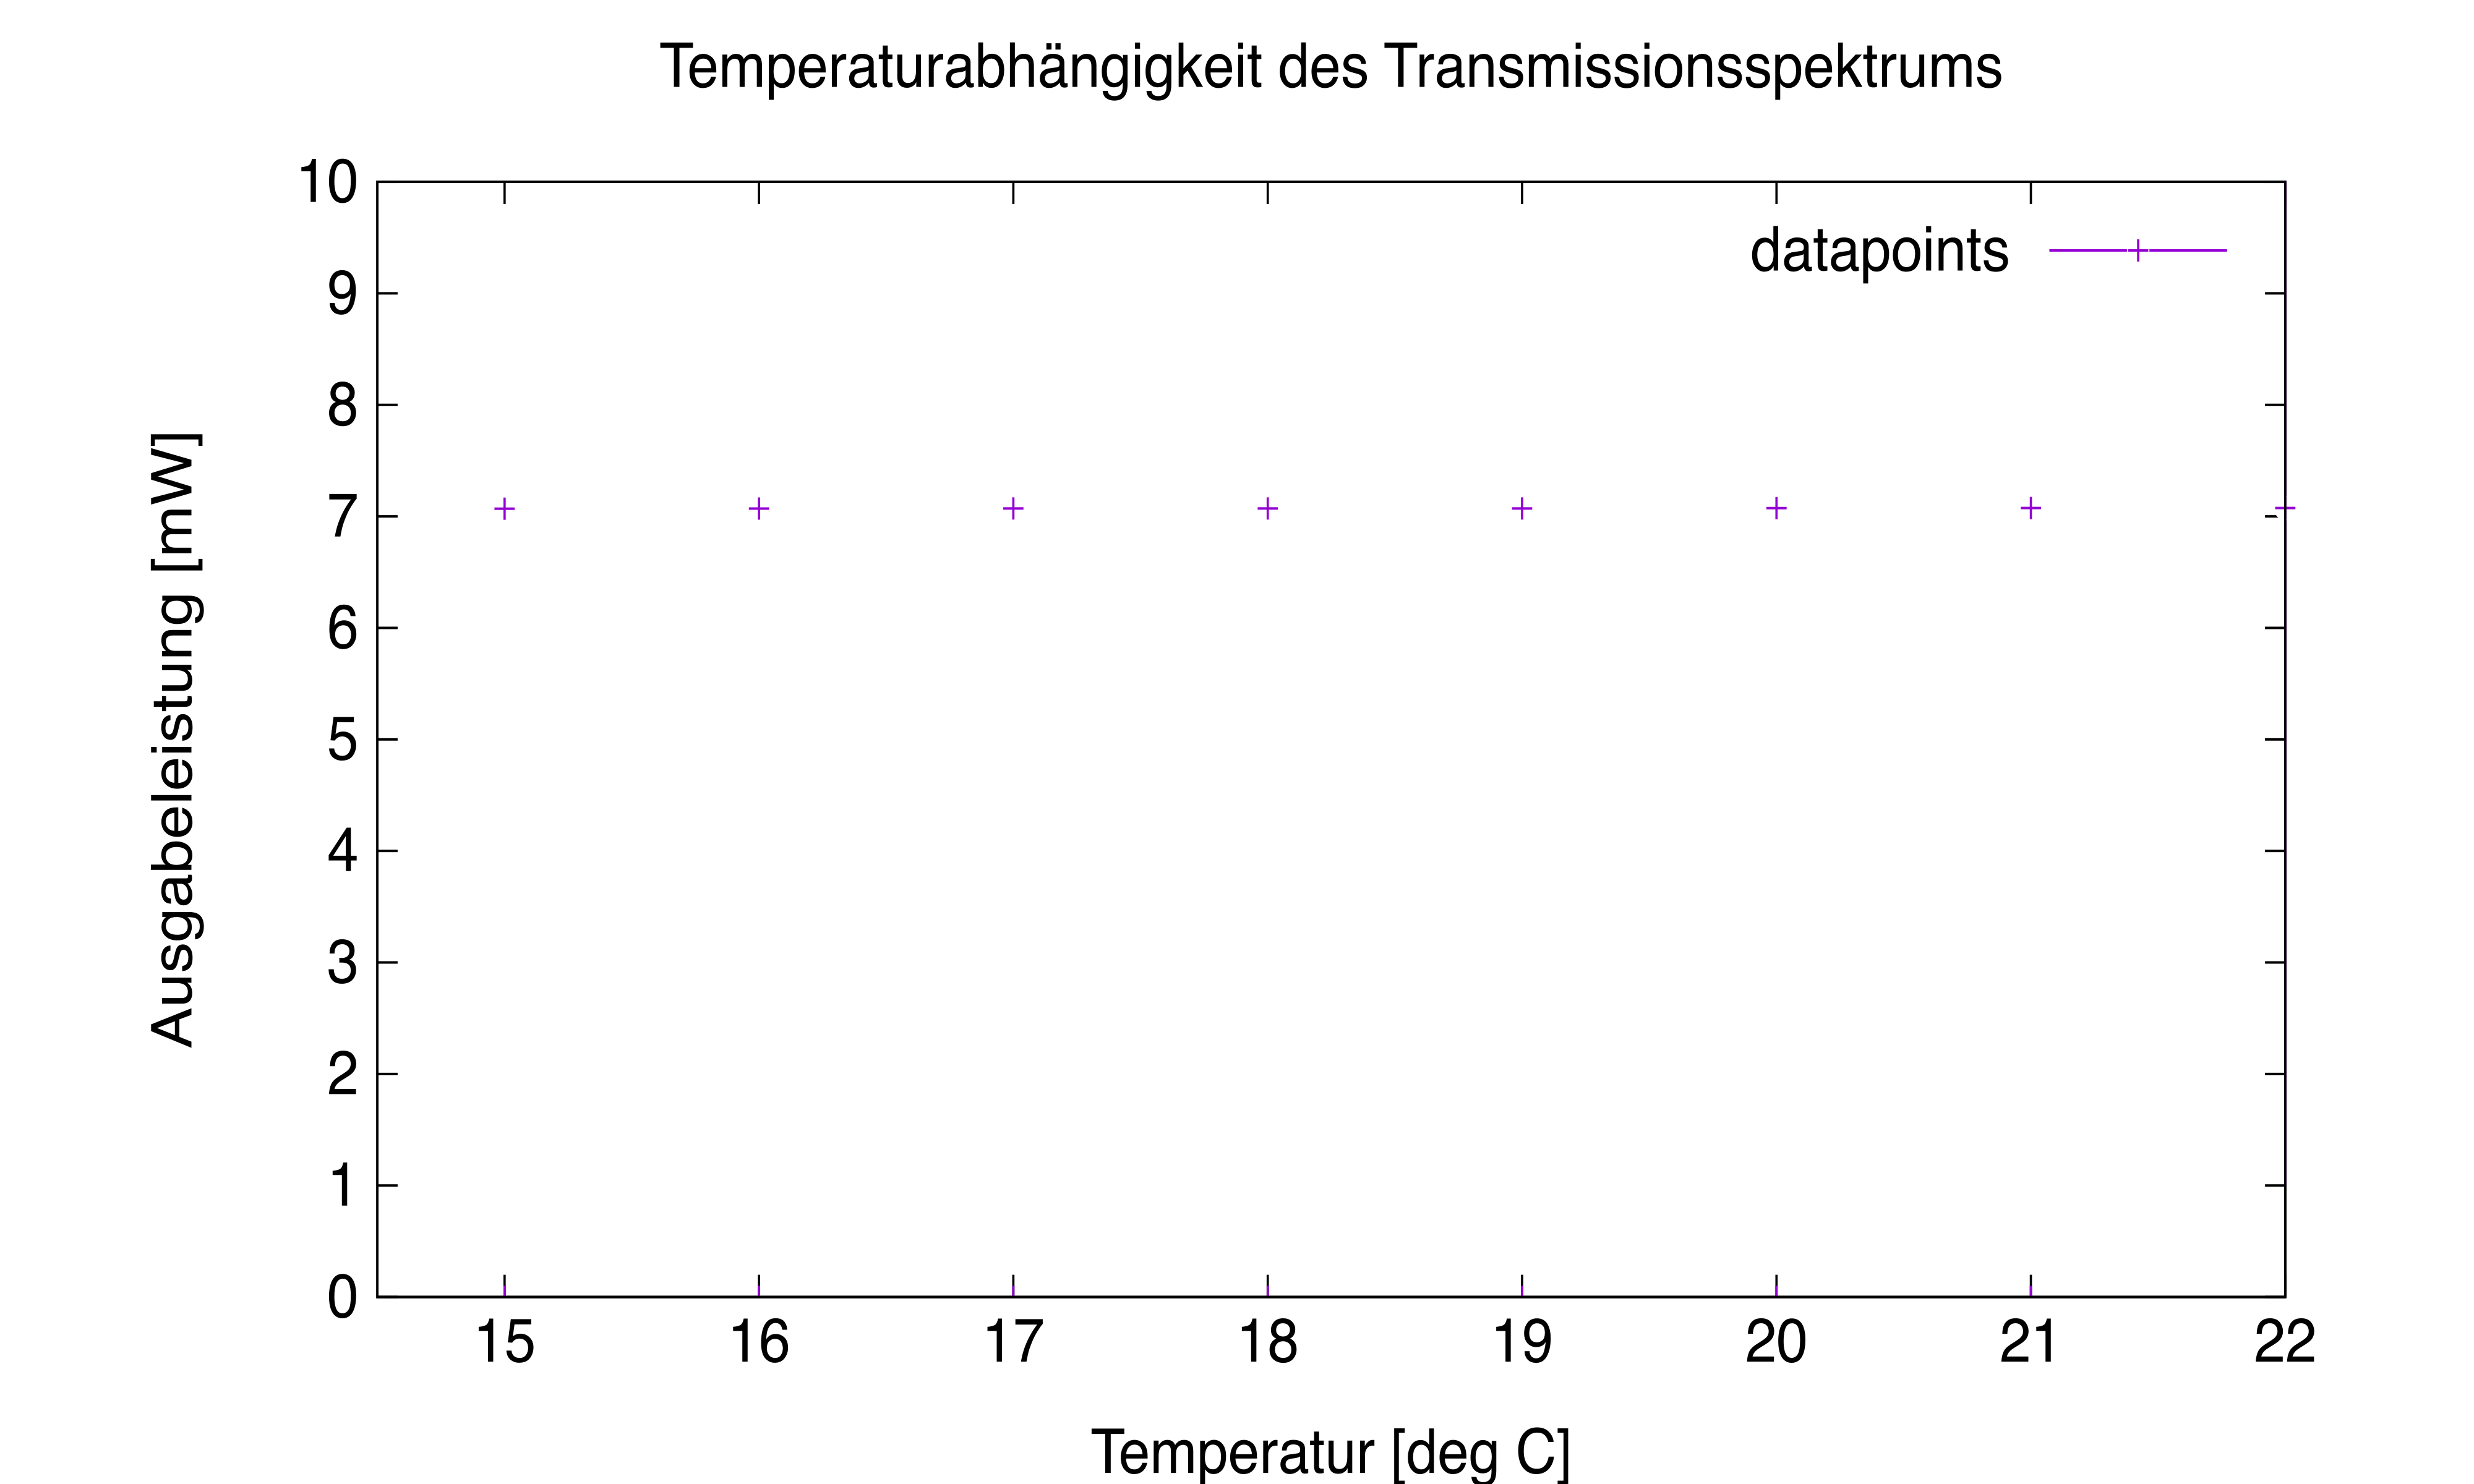
\includegraphics[width=8cm]{Bilddateien/TransmissionOverTemperatureSuS.png}
                    \caption{Transmission über Temperatur. Der Zusammenhang sieht linear aus.}
                    \label{fig:TransmissionOverTemperatureSuS}
                \end{figure}
                Wir haben uns vom Tutor erklären lassen, daß der Sensor übersättigt war. 
                \marginnote{10:25}
                Starte neu.
            \subparagraph*{Unterabschnit 1.2}
            

        \paragraph*{Versuchsteil 2}

            
        \paragraph*{Versuchsteil 3}


        \paragraph*{Versuchsteil 4}

        
        \paragraph*{Versuchsteil 5}

            \subparagraph*{Unterabschnit 5.1}

            \subparagraph*{Unterabschnit 5.2}

            \subparagraph*{Unterabschnit 5.3}

            \subparagraph*{Unterabschnit 5.4}

            \subparagraph*{Unterabschnit 5.5}
    
            
        \paragraph*{Versuchsteil 6}

        
        \paragraph*{Versuchsteil 7}

            \subparagraph*{Unterabschnit 7.1}

            \subparagraph*{Unterabschnit 7.2}
            

        \paragraph*{Dateinamen}

        \begin{table}[H]
            \centering
            \begin{tabular}{p{4cm}|c|p{6cm}}
                \textbf{Dateiname} & \textbf{Nutzbarkeit} & \textbf{Bedeutung} \\
                \hline\hline
                \texttt{Exp1} & & \\
                \texttt{Exp2} & & \\
                \hline
                \texttt{AutoShim1} & x & Testlauf des \emph{auto-shimming} \\
                \texttt{AutoShim2} & & \\
                \hline
                \texttt{Explore-FID1} & & Testaufnahme unter Varrierung von \emph{recieve gain} \\
                \texttt{Explore-FID2} & & \\
                \texttt{Explore-FID3} & & \\
                \hline
                \texttt{C-Opti} & x & Wert $10.8$ war bereits optimiert. \\
                \hline
                \texttt{B1DurationFast} & & \\
                \texttt{B1Opti} & & \\
                \hline
                \texttt{FID-Characterize1} & x & Optimale Einstellungen mit \emph{pulse duration} auf $25\si{\ms}$\\
                \texttt{FID-Characterize2} & & \\
                \hline
                \texttt{T1-Bp-10steps} & & Spin-Gitter-Relaxion im Polarisationsfeld \\
                \texttt{T1-Bp-20steps} & & \\
                \hline
                \texttt{Echo-optimal-}\texttt{positive-multi-average} & & \\
            \end{tabular}
        \end{table}
\end{document}